% geometry_and_trigonometry:x04 GDC:NO
\begin{question}
  \hspace*{\fill} [Note Maximale: ?]\par
  \medskip
  \noindent La figure qui suit représente en pentagone $ABCDE$. tel que:\par
  \noindent $AB = 9,2\,cm,  BC = 3,2\,cm, BD = 7,1\,cm, \angle\,AED = 110^\circ, \angle\,ADE = 52^\circ,$ et $\angle\,ABD = 60^\circ$.\par
  \medskip
  \begin{center} % or flushleft or flushright
    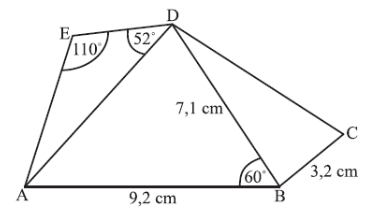
\includegraphics[scale=0.4]{figure_x4}\par
  \end{center} % or flushleft or flushright
  \begin{enumerate}[label=(\alph*)]
    \item Trouvez $AD$.\hspace*{\fill} [?]
    \item Trouvez $DE$.\hspace*{\fill} [?]
    \item L'aire du triangle $bcd$ est $5,68\,cm^2$. Trouvez $\angle\,DBC$\hspace*{\fill} [?]
    \item Trouvez $AC$.\hspace*{\fill} [?]
  \end{enumerate}
\end{question}
